% !TEX root = ./document.tex

\documentclass[a4paper, spanish]{article}

\usepackage{mystyle}
\usepackage{myvars}

\begin{document}

  \maketitle

  \begin{itemize}
    \item \textbf{Archivo}: \texttt{tuberculo.sf3}
    \item \textbf{Serie}: Número de casos registrados semanalmente de tuberculosis respiratoria en España, entre los años $1982$ y $1991$ (el primer dato corresponde al número de casos registrados desde el \emph{$1$ de Enero de $1982$} al \emph{$7$ de Enero de $1982$}).
    \begin{itemize}
      \item $\{X_t\}$ Serie Original.
      \item $\{Y_t\}$ Serie del número de casos en periodos de cuatro semanas sucesivos.
    \end{itemize}
  \end{itemize}

  \section{Describir estas dos series ($\{Y_t\}$ puede crearse con el \texttt{proc expand} de \emph{SAS}), indicando claramente para cada una de ellas qué frecuencias elegiríais a priori para ajustar un modelo con tendencia polinómica más ondas.}
  \label{sec:a}


    \begin{figure}
      \centering
      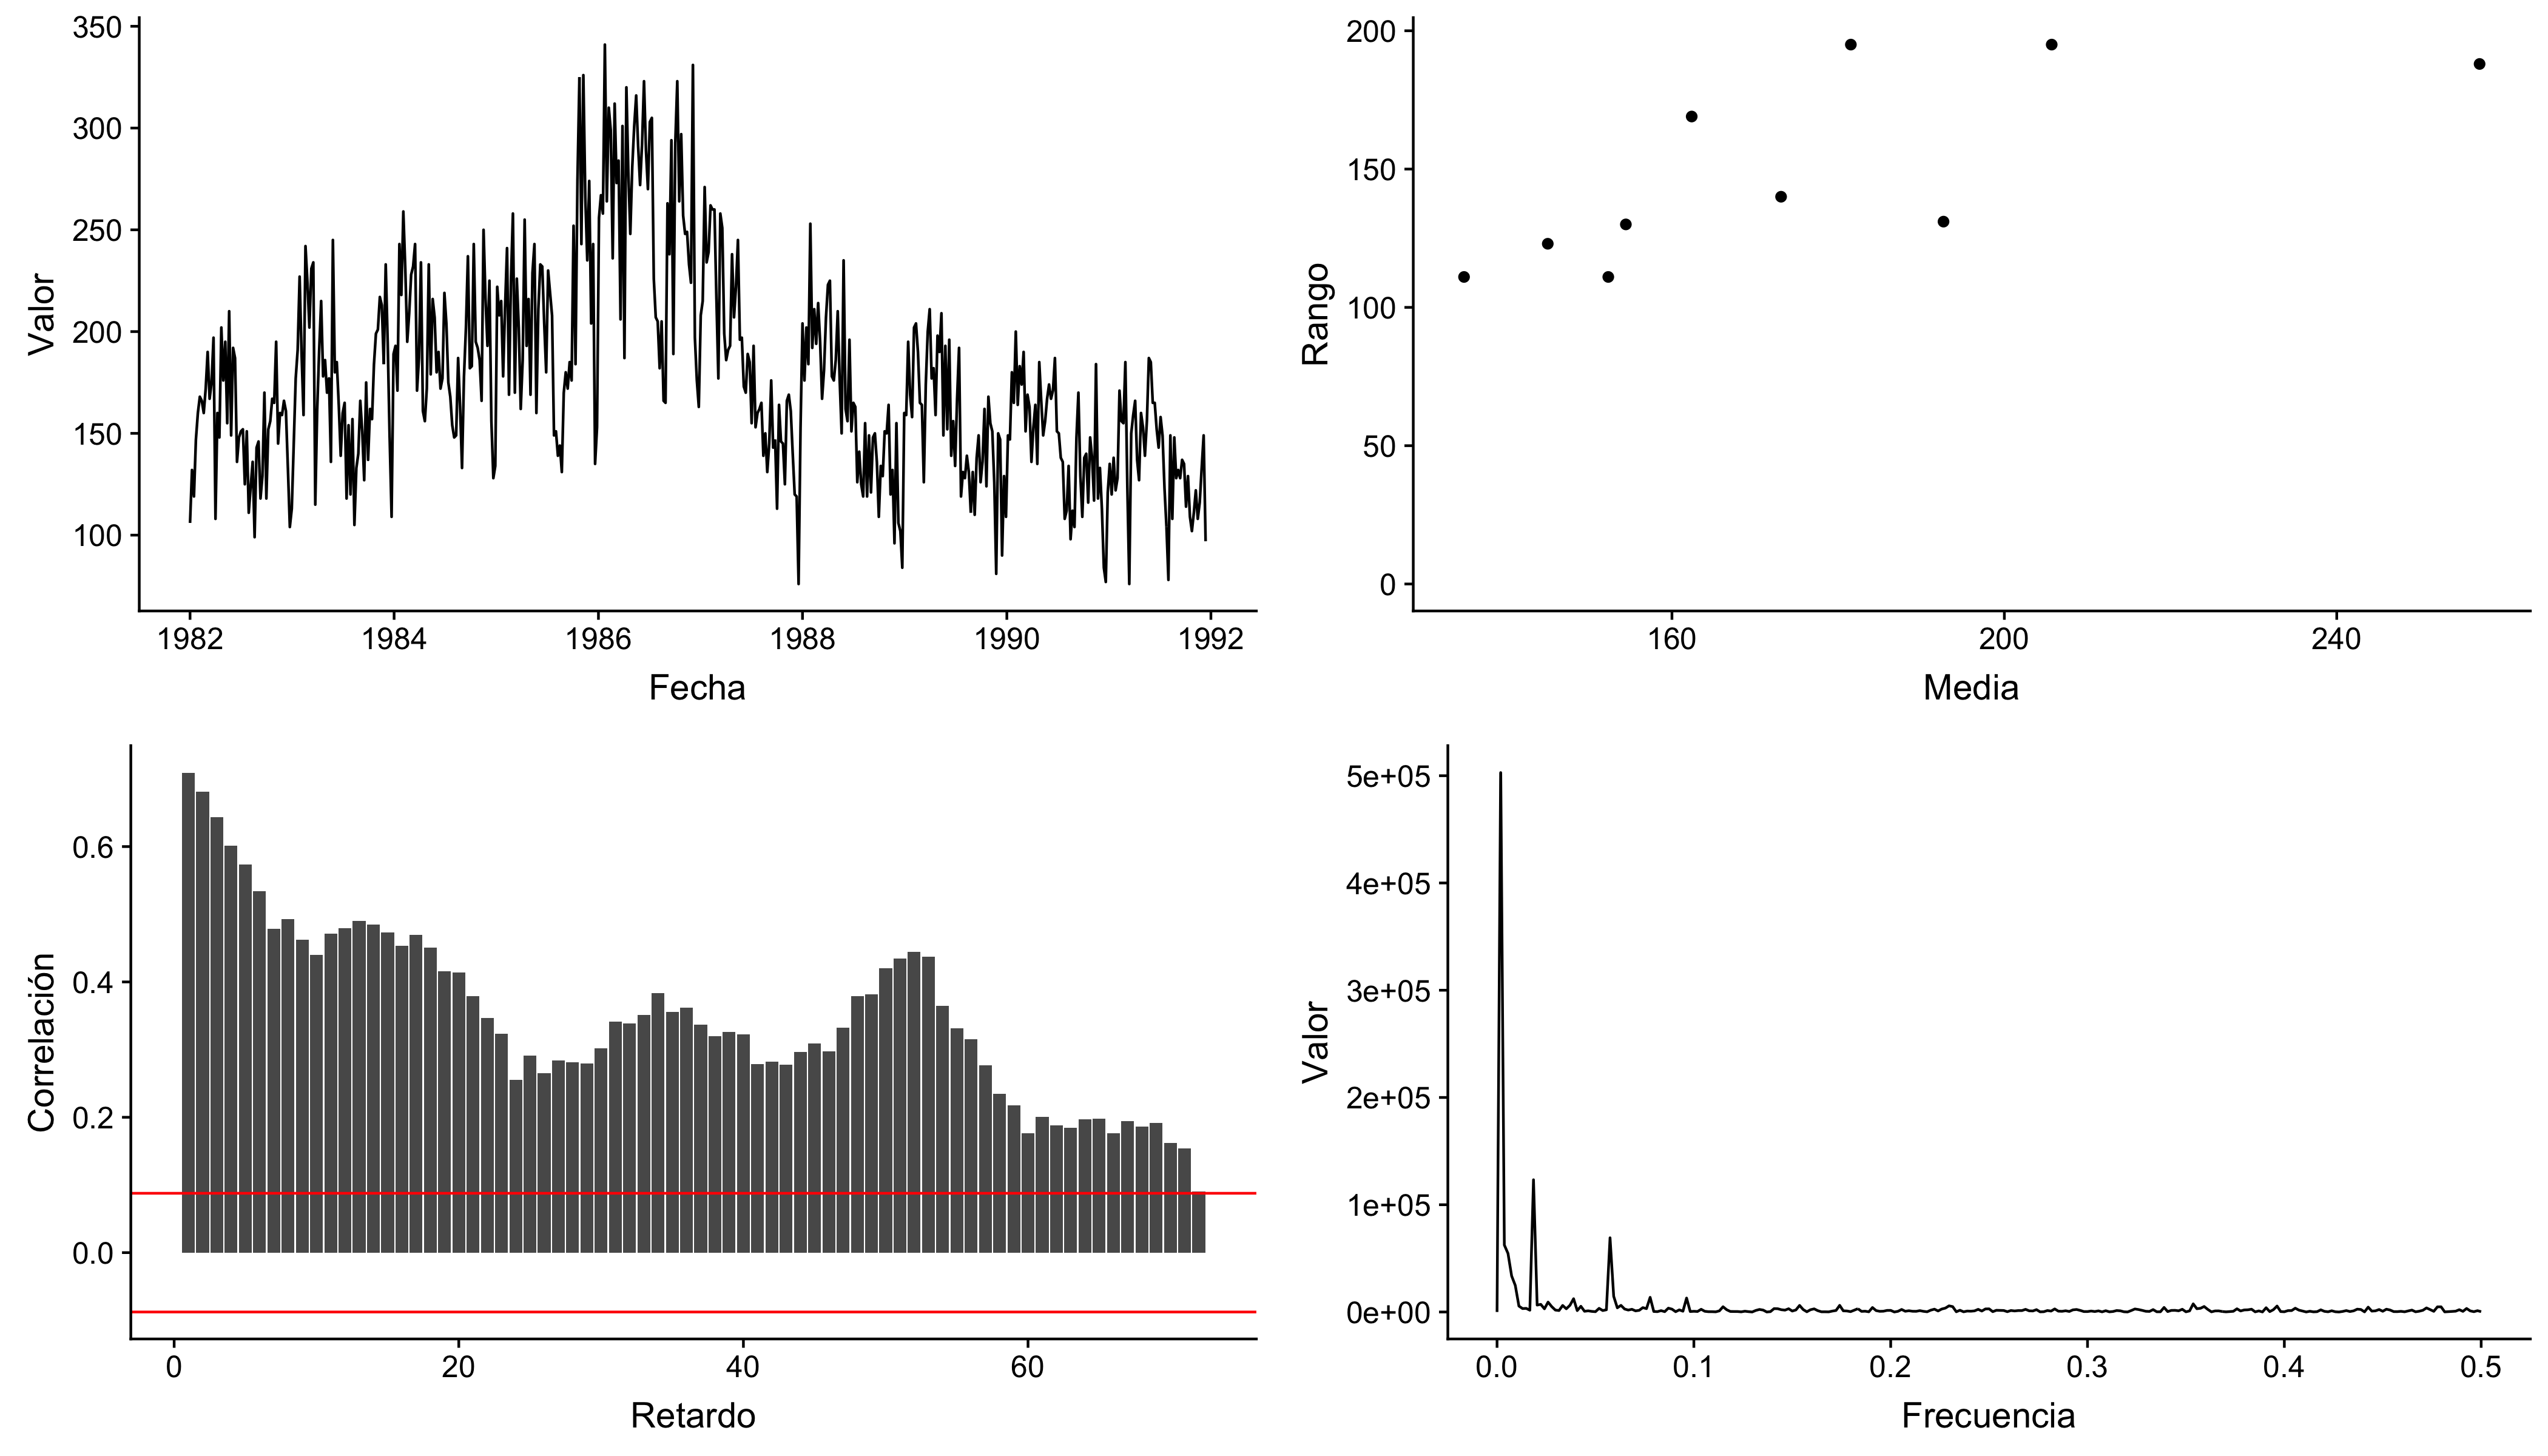
\includegraphics[width=.75\linewidth]{semanal}
      \caption{[TODO]}
      \label{fig:fitted}
    \end{figure}

    \paragraph{}
    [TODO]


    \begin{figure}
      \centering
      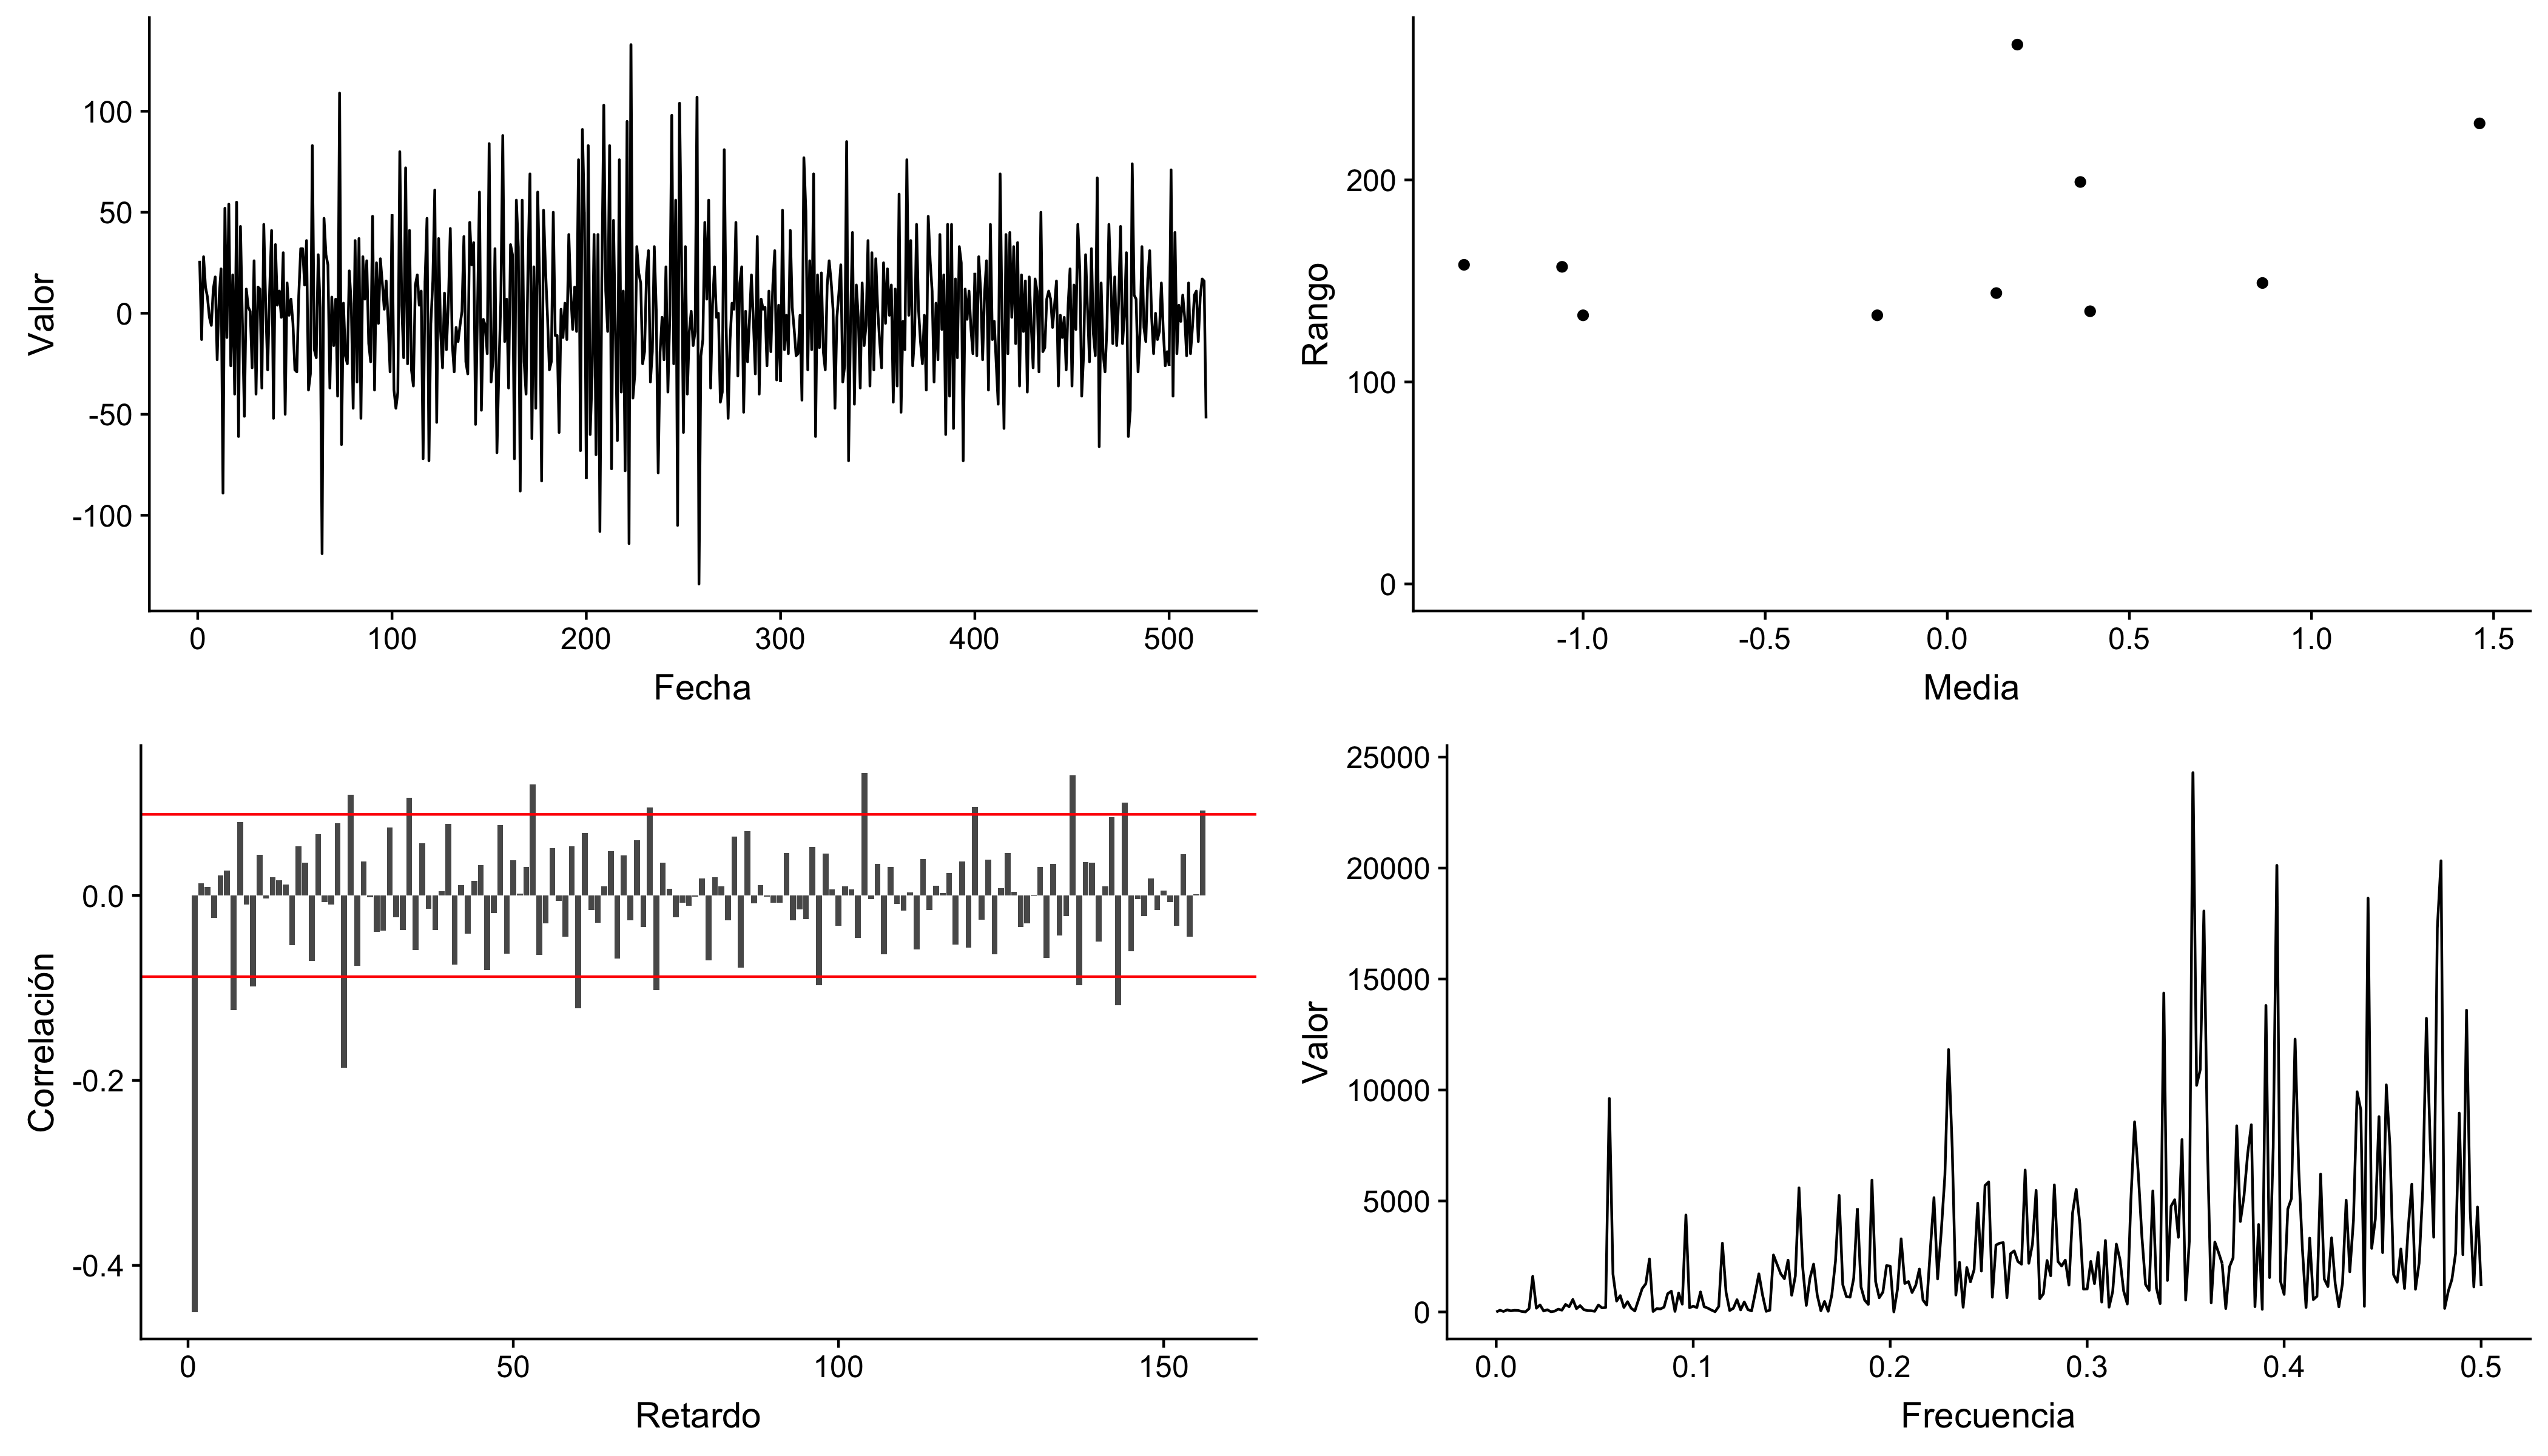
\includegraphics[width=.75\linewidth]{semanal-diff}
      \caption{[TODO]}
      \label{fig:fitted}
    \end{figure}

    \paragraph{}
    [TODO]


    \begin{figure}
      \centering
      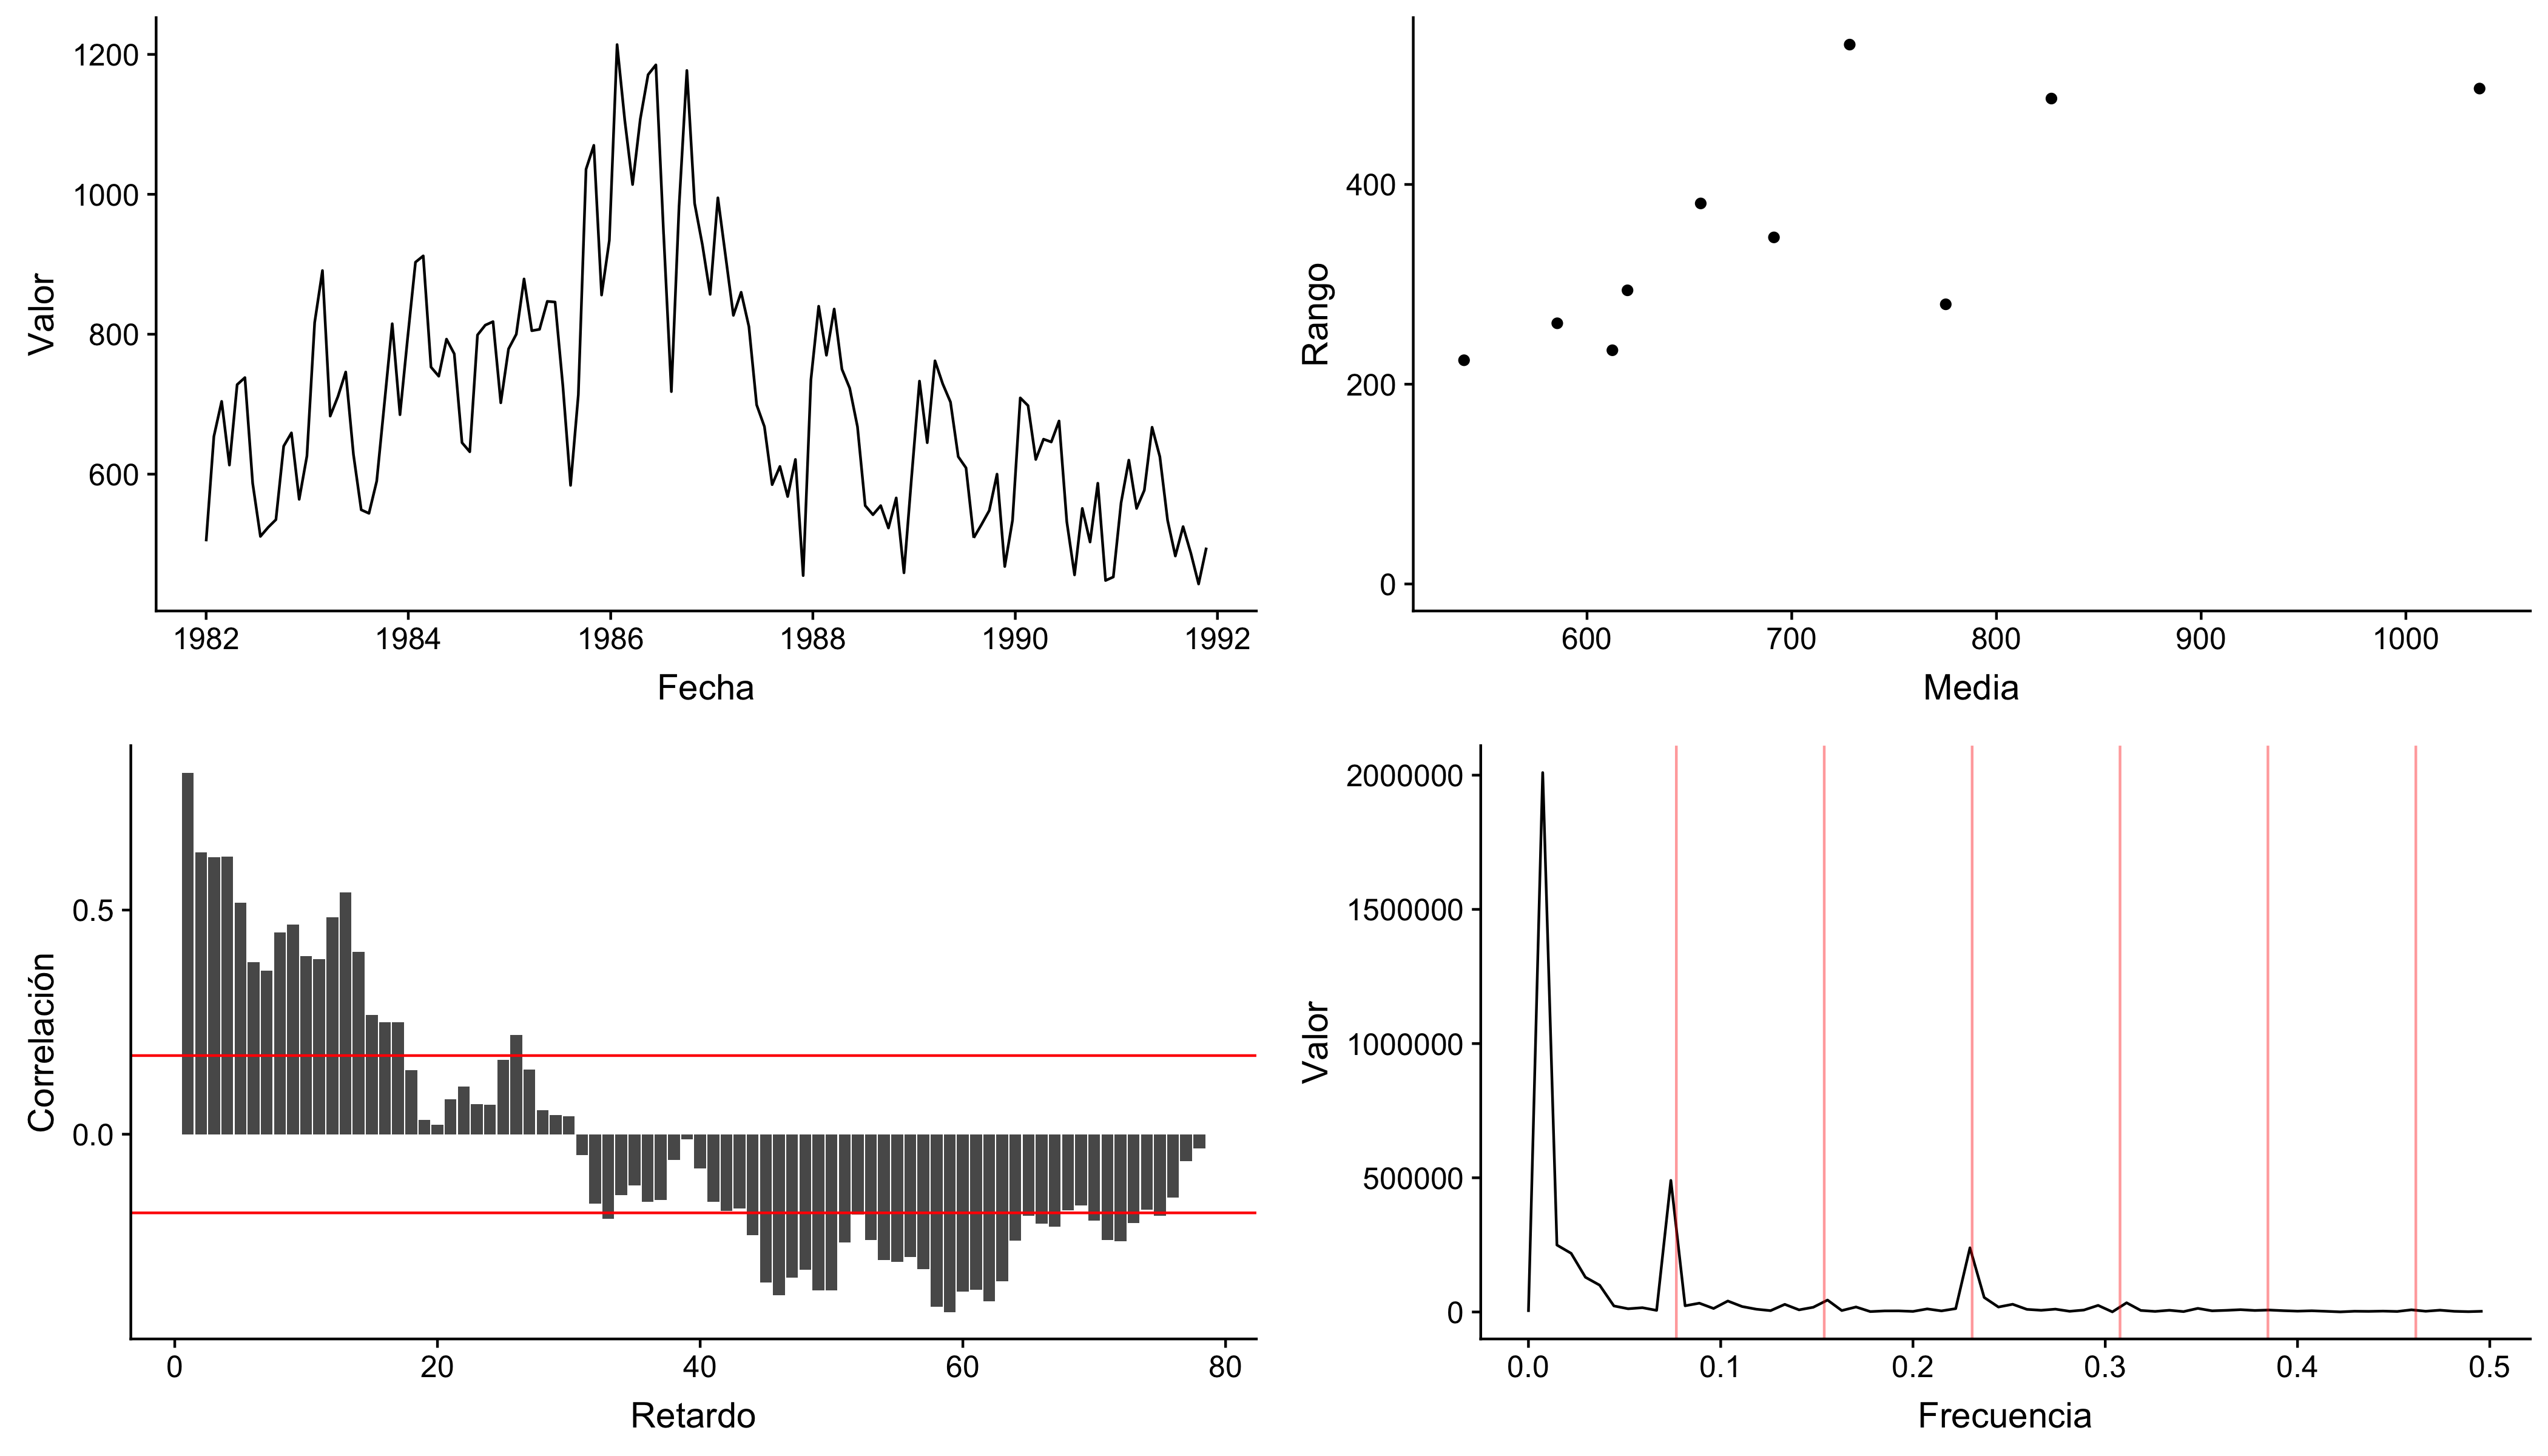
\includegraphics[width=.75\linewidth]{semanal4}
      \caption{[TODO]}
      \label{fig:fitted}
    \end{figure}

    \paragraph{}
    [TODO]


    \begin{figure}
      \centering
      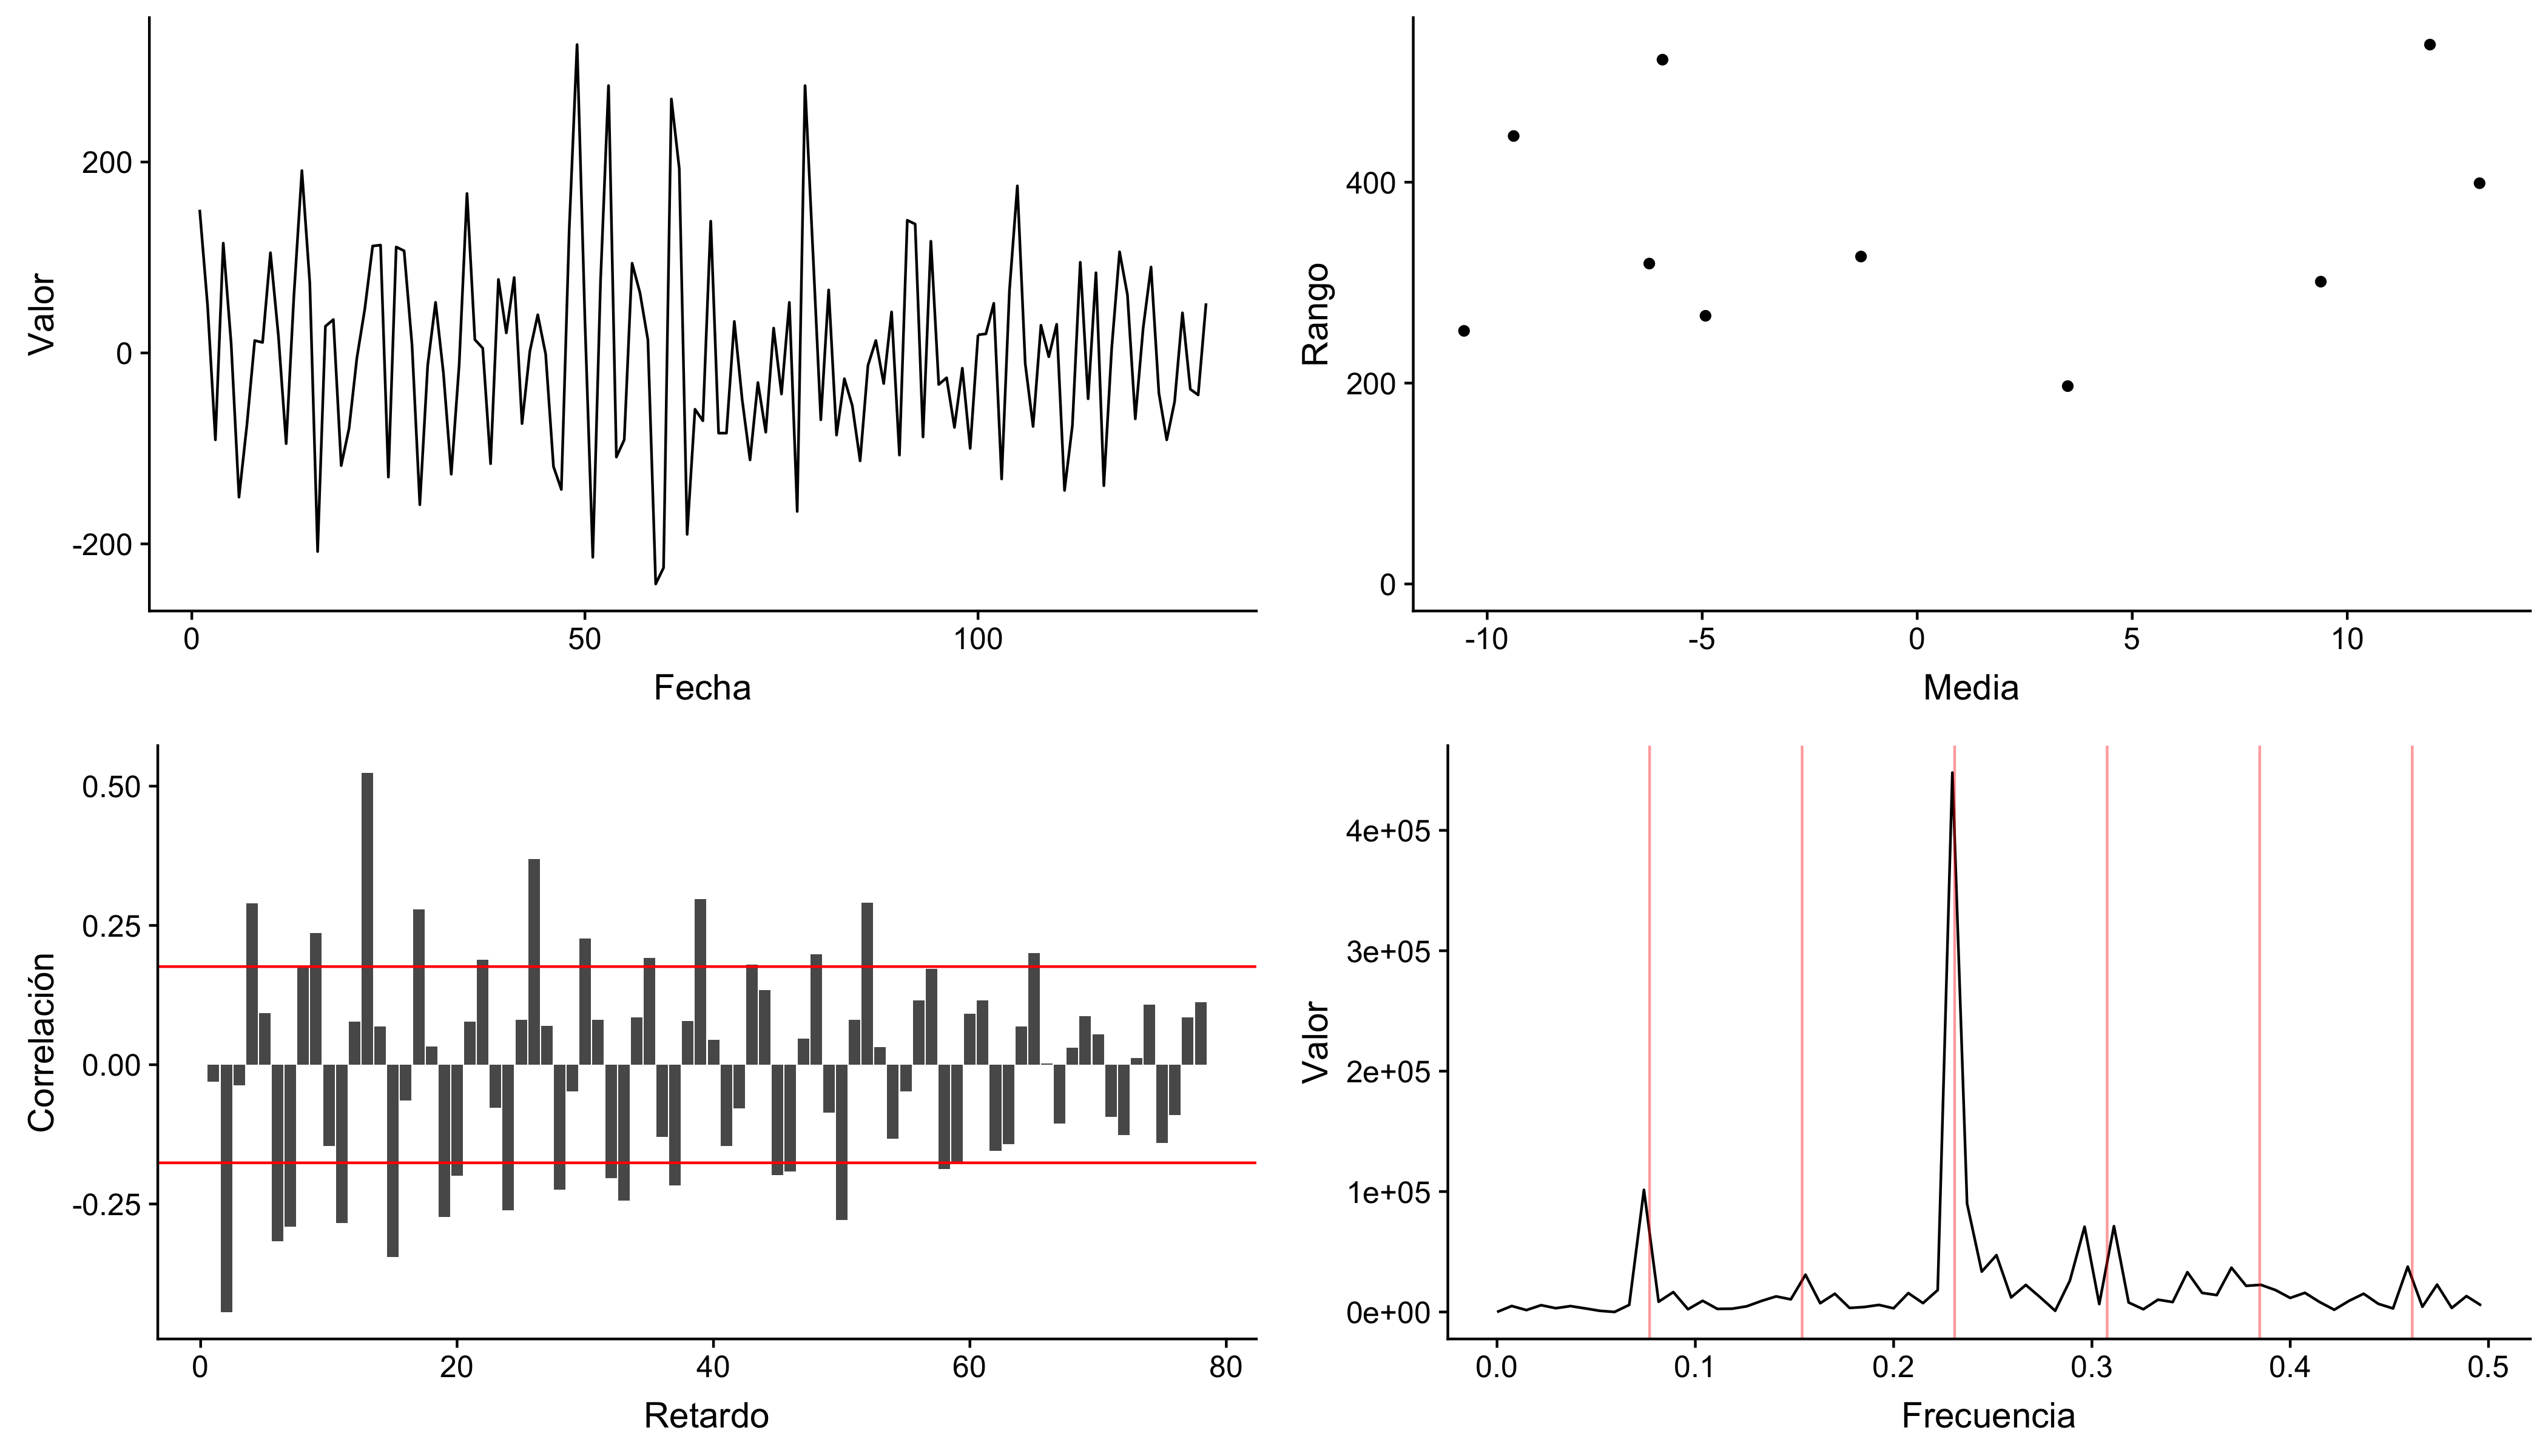
\includegraphics[width=.75\linewidth]{semanal4-diff}
      \caption{[TODO]}
      \label{fig:fitted}
    \end{figure}

    \paragraph{}
    [TODO]

    \begin{figure}[h]
      \centering
      \inputminted{SAS}{./res/code/a-01-data.sas}
      \caption{[TODO]}
      \label{code:a_data}
    \end{figure}

    \paragraph{}
    [TODO]

    \begin{figure}[h]
      \centering
      \inputminted{SAS}{./res/code/a-02-expand.sas}
      \caption{[TODO]}
      \label{code:a_expand}
    \end{figure}

    \paragraph{}
    [TODO]

    \begin{figure}[h]
      \centering
      \inputminted{SAS}{./res/code/a-03-describe-x.sas}
      \caption{[TODO]}
      \label{code:a_describe_x}
    \end{figure}

    \paragraph{}
    [TODO]

    \begin{figure}[h]
      \centering
      \inputminted{SAS}{./res/code/a-03-describe-y.sas}
      \caption{[TODO]}
      \label{code:a_describe_y}
    \end{figure}

    \paragraph{}
    [TODO]

  \section{Ajustar por suavizado exponencial, con el \texttt{proc esm}, los tres modelos que se consideren más apropiados para la serie $\{Y_t\}$ y comprobar su adecuación.}
  \label{sec:b}

    \paragraph{}
    [TODO]

    \begin{figure}[h]
      \centering
      \inputminted{SAS}{./res/code/b-01-esm-1.sas}
      \caption{[TODO]}
      \label{code:b_esm_1}
    \end{figure}

    \paragraph{}
    [TODO]

    \begin{figure}[h]
      \centering
      \inputminted{SAS}{./res/code/b-01-esm-2.sas}
      \caption{[TODO]}
      \label{code:b_esm_2}
    \end{figure}

    \paragraph{}
    [TODO]

    \begin{figure}[h]
      \centering
      \inputminted{SAS}{./res/code/b-01-esm-3.sas}
      \caption{[TODO]}
      \label{code:b_esm_3}
    \end{figure}

    \paragraph{}
    [TODO]


  \section{Elegir el modelo que se considere más apropiado entre los tres del apartado \ref{sec:b} y con ese modelo dar las predicciones para las próximas $6$ observaciones. Justificar la elección del modelo.}
  \label{sec:c}

    \paragraph{}
    [TODO]

    \begin{figure}[h]
      \centering
      \inputminted{SAS}{./res/code/c-01-prediction.sas}
      \caption{[TODO]}
      \label{code:c_prediction}
    \end{figure}

    \paragraph{}
    [TODO]

  \section{Utilizando en el ajuste solamente los datos hasta el final de $1990$ que no incluyan ningún caso de $1991$, calcular los errores de predicción para el año $1991$ y su correspondiente $SSE_p$ (suma de $s$ errores al cuadrado correspondientes a predicciones $\{1, 2, ..., s\}$ pasos hacia adelante) para los tres modelos del apartado \ref{sec:b}. Comentar si la elección hecha en el apartado \ref{sec:c} está de acuerdo con los resultados obtenidos en este caso al comparar la capacidad de predicción de los distintos modelos para el año $1991$. Adjuntad el programa con el lenguaje control que hayáis utilizado en este apartado.}
  \label{sec:d}

    \paragraph{}
    [TODO]

    \begin{figure}[h]
      \centering
      \inputminted{SAS}{./res/code/d-01-prediction-error-esm-1.sas}
      \caption{[TODO]}
      \label{code:d_prediction_error_esm_1}
    \end{figure}

    \paragraph{}
    [TODO]

    \begin{figure}[h]
      \centering
      \inputminted{SAS}{./res/code/d-01-prediction-error-esm-2.sas}
      \caption{[TODO]}
      \label{code:d_prediction_error_esm_2}
    \end{figure}

    \paragraph{}
    [TODO]

    \begin{figure}[h]
      \centering
      \inputminted{SAS}{./res/code/d-01-prediction-error-esm-3.sas}
      \caption{[TODO]}
      \label{code:d_prediction_error_esm_3}
    \end{figure}

    \paragraph{}
    [TODO]


  \section{Obtener con el \texttt{proc forecast} de \emph{SAS} el $SSE_p$ para el modelo de \emph{Winter Multiplicativo} con las mismas constantes de suavizado y los valores iniciales de los parámetros lo más próximos posible a los obtenidos en el apartado \ref{sec:d} con el \texttt{proc esm} para este modelo. Adjuntar el programa con el lenguaje control que hayáis utilizado para obtenerlo.}
  \label{sec:e}

    \paragraph{}
    [TODO]

    \begin{figure}[h]
      \centering
      \inputminted{SAS}{./res/code/e-01-prediction-error-forecast-1.sas}
      \caption{[TODO]}
      \label{code:e_prediction_error_forecast_1}
    \end{figure}

    \paragraph{}
    [TODO]

    \begin{figure}[h]
      \centering
      \inputminted{SAS}{./res/code/e-01-prediction-error-forecast-2.sas}
      \caption{[TODO]}
      \label{code:e_prediction_error_forecast_2}
    \end{figure}

    \paragraph{}
    [TODO]

    \begin{figure}[h]
      \centering
      \inputminted{SAS}{./res/code/e-01-prediction-error-forecast-3.sas}
      \caption{[TODO]}
      \label{code:e_prediction_error_forecast_3}
    \end{figure}

    \paragraph{}
    [TODO]


  \section{Ajustar un modelo para la serie $\{ Xt \}$ con el módulo \texttt{Time Series Forecasting System} de \emph{SAS} razonando porqué se ha elegido. Utilizar el modelo elegido para predecir valores futuros de esta serie y establecer la comparación con los seis valores obtenidos en el apartado \ref{sec:c} junto con sus bandas de predicción.}
  \label{sec:f}

    \paragraph{}
    [TODO]


\end{document}
